\section{System's perspective} \label{section:System perspective}
\subsection{Design}
The Minitwit application is a simple application allowing users to post messages, see messages posted by others and follow other users in order to specifically see what they post.

The application is implemented in Java with the Spark Framework and a MySQL database. Java was chosen since it is platform independent and a popular language, meaning that extensive documentation is available and it would be easy for a future team to inherit the code. Spark was chosen as it is a lightweight framework like Flask, which was used for the inherited Minitwit system. Spark also has a reasonable learning curve and is straight forward to use for an application the size of Minitwit. The frontend consist of HTML templates connected to the backend using the template engine Jinjava, chosen to mimic the python Minitwit with little to no changes. 

MySQL was chosen for persistent data storage due to its high performance, wide adoption rate, indices and familiarity to the team. Furthermore, the relational model fits the Minitwit data well and \hyperref[fig:classDiagramModel]{figure \ref{fig:databaseDiagram}} depicts the design of the database.
\begin{figure}[H]
    \centering
    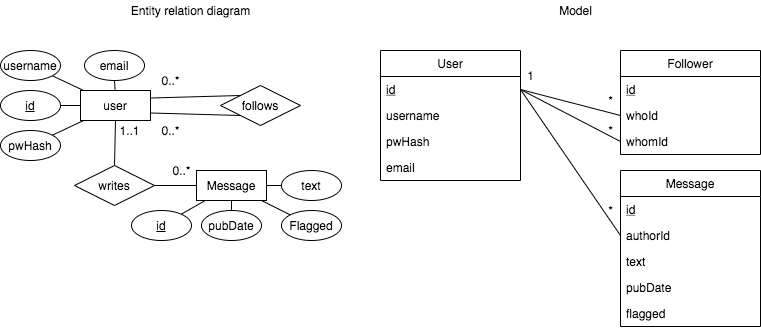
\includegraphics[width=1\textwidth]{report/images/Diagrams-DB.png}
    \caption{Entity relation diagram and diagram of model presenting the design of the database tables.}
    \label{fig:databaseDiagram}
\end{figure} 
\vspace{3mm}

\noindent
The ORM tool used is NORM, which is a lightweight ORM that does not require the complex markdown files that tools like Hibernate or JPA introduce. It is suitable for smaller projects with simple models and therefore fulfills the requirements of the Minitwit application. As an ORM tool NORM is not perfect as some queries still requires writing sql, like when joining or adding indexes.

Hibernate was implemented on branch feature/Hibernate\footnote{\url{https://github.com/DevOps2021-gb/devops2021/tree/feature/Hibernate}} as a test to see if it would be a better fit. Unfortunately, it turned out that the tool did not deliver on its promises and actually did not support some union queries, meaning that it only introduced more unnecessary complexity without adding any benefits. Furthermore, it complicated database joins which are needed for Minitwit. We therefore decided to stick with NORM.

The application is hosted on DigitalOcean. Measures taken to ensure availability and maintenance, monitoring with Prometheus and Grafana and logging using an EFK-stack, are described later.

\newpage
\subsection{Architecture}

\hyperref[fig:componentDiagram]{Figure \ref{fig:componentDiagram}} shows the different components of the application and how they are connected.
\begin{figure}[H]
    \centering
    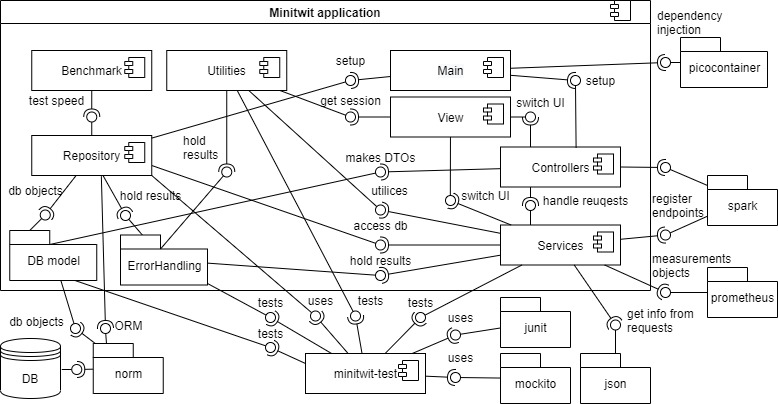
\includegraphics[width=1\textwidth]{images/Diagrams-Development_view_component_diagram.jpg}
    \caption{Component diagram of the entire Minitwit application, development view}
    \label{fig:componentDiagram}
\end{figure}

\subsubsection{Main}
Main is the system entry point and allows specification of which database to use. Main starts monitoring and logging services and defines the number of threads to use. \hyperref[fig:classDiagramMain]{Figure \ref{fig:classDiagramMain}} presents a class diagram. 
\begin{figure}[H]
    \centering
    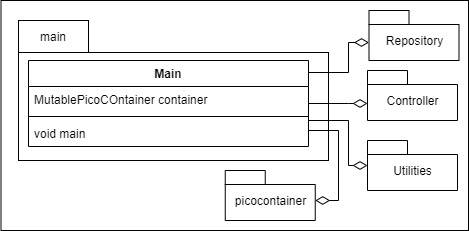
\includegraphics[width=0.5\textwidth]{images/class_diagram_main.jpg}
    \caption{Class diagram for main, logical view}
    \label{fig:classDiagramMain}
\end{figure}

\subsubsection{Utilities}
Utilities, shown in \hyperref[fig:classDiagramUtilities]{figure \ref{fig:classDiagramUtilities}}, contains helper methods like hashing, formatting dates and JSON, and houses Request, Response and Session wrapper objects to use with Spark.
\begin{figure}[H]
    \centering
    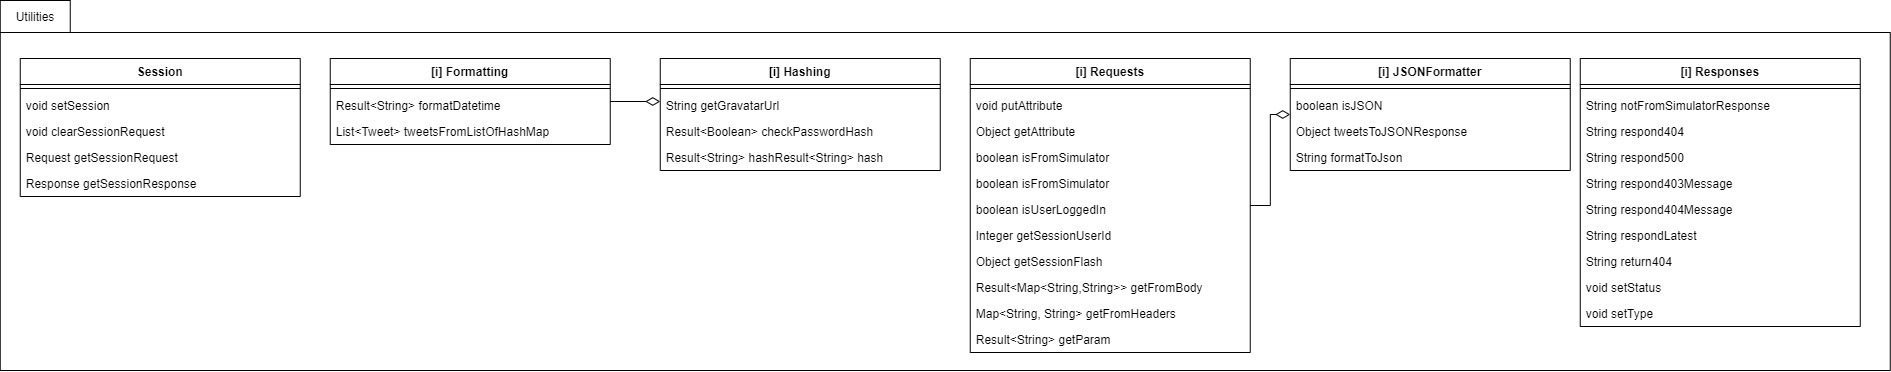
\includegraphics[width=1.0\textwidth]{images/class_diagram_utilities.jpg}
    \caption{Class diagram utilities, logical view}
    \label{fig:classDiagramUtilities}
\end{figure}

\subsubsection{Error handling}
Error handling contains objects used to wrap results of computations that can result in exceptions, allowing for better error handling and reduction of try-catch-statements. A class diagram is presented in  \hyperref[fig:classDiagramErrorhandling]{figure \ref{fig:classDiagramErrorhandling}}.
\begin{figure}[H]
    \centering
    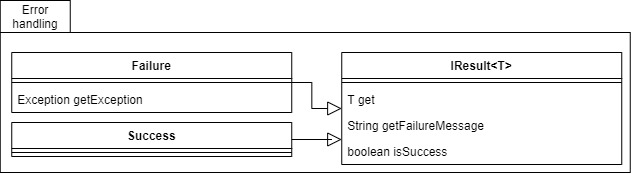
\includegraphics[width=0.8\textwidth]{images/class_diagram_errorhandling.jpg}
    \caption{Class diagram for Error handling, logical view}
    \label{fig:classDiagramErrorhandling}
\end{figure}

\subsubsection{Controllers}
Controllers handles the API endpoints the application provides by mapping post and get request to appropriate methods. The class diagram can be seen in \hyperref[fig:classDiagramControllers]{figure \ref{fig:classDiagramControllers}}.
\begin{figure}[H]
    \centering
    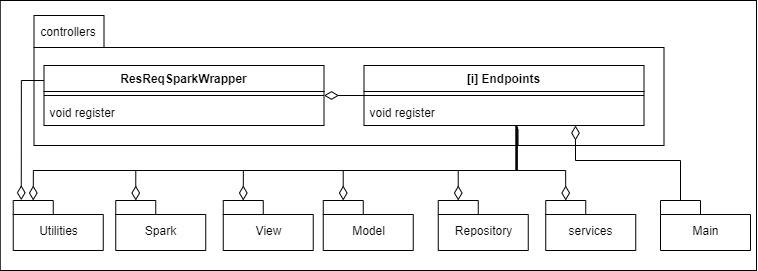
\includegraphics[width=1.0\textwidth]{images/class_diagram_controllers.jpg}
    \caption{Class diagram for controllers, logical view}
    \label{fig:classDiagramControllers}
\end{figure}

\subsubsection{View}
View contains code for rendering and redirecting between pages of Minitwit. Pages are rendered html-templates. The class diagram can be seen in \hyperref[fig:classDiagramView]{figure \ref{fig:classDiagramView}}.
\begin{figure}[H]
    \centering
    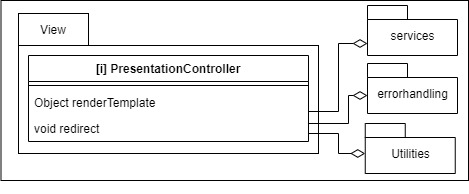
\includegraphics[width=0.6\textwidth]{images/class_diagram_view.jpg}
    \caption{Class diagram for View, logical view}
    \label{fig:classDiagramView}
\end{figure}

\subsubsection{Services}
Services includes functions executing requests and responses along with code for gathering and printing information to be used by the monitoring and logging services.
%Services includes code for maintenance, which uses Prometheus library to store the values Prometheus should collect, and the log service, which prints in a manner easy to filter for in Kibana. Services also includes functions executing the requests and responses.\\
Class diagram presented in \hyperref[fig:classDiagramServices]{figure \ref{fig:classDiagramServices}}.
 \begin{figure}[H]
    \centering
    \hspace*{-1.1in}
    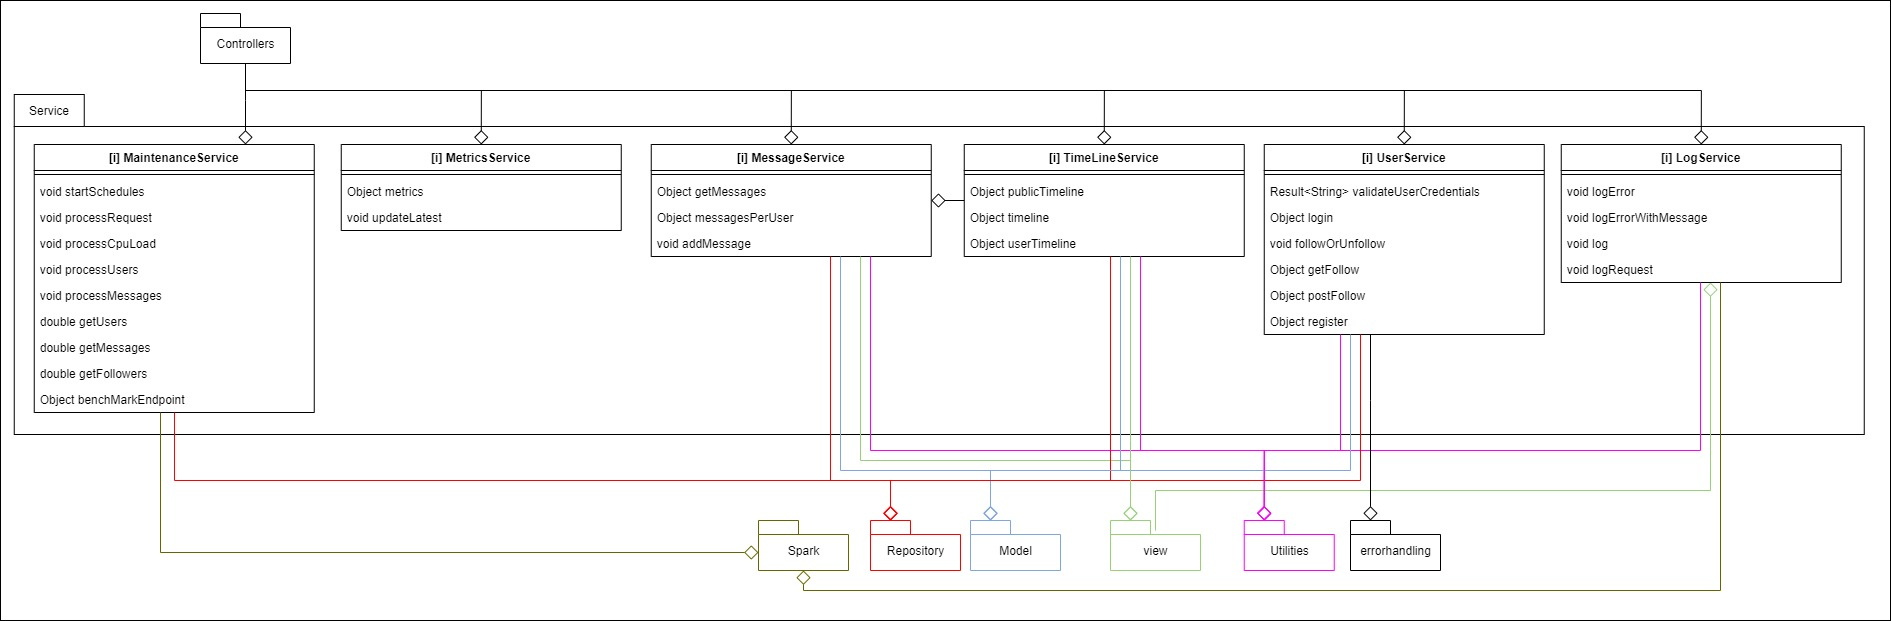
\includegraphics[width=1.35\textwidth]{images/class_diagram_services.jpg}
    \caption{Class diagram services, logical view}
    \label{fig:classDiagramServices}
\end{figure}

\subsubsection{Repository}
Repository includes code for starting the database and executing queries needed by the services. Class diagram can be seen in \hyperref[fig:classDiagramRepository]{figure \ref{fig:classDiagramRepository}}.
\begin{figure}[H]
    \centering
    \hspace*{-0.5in}
    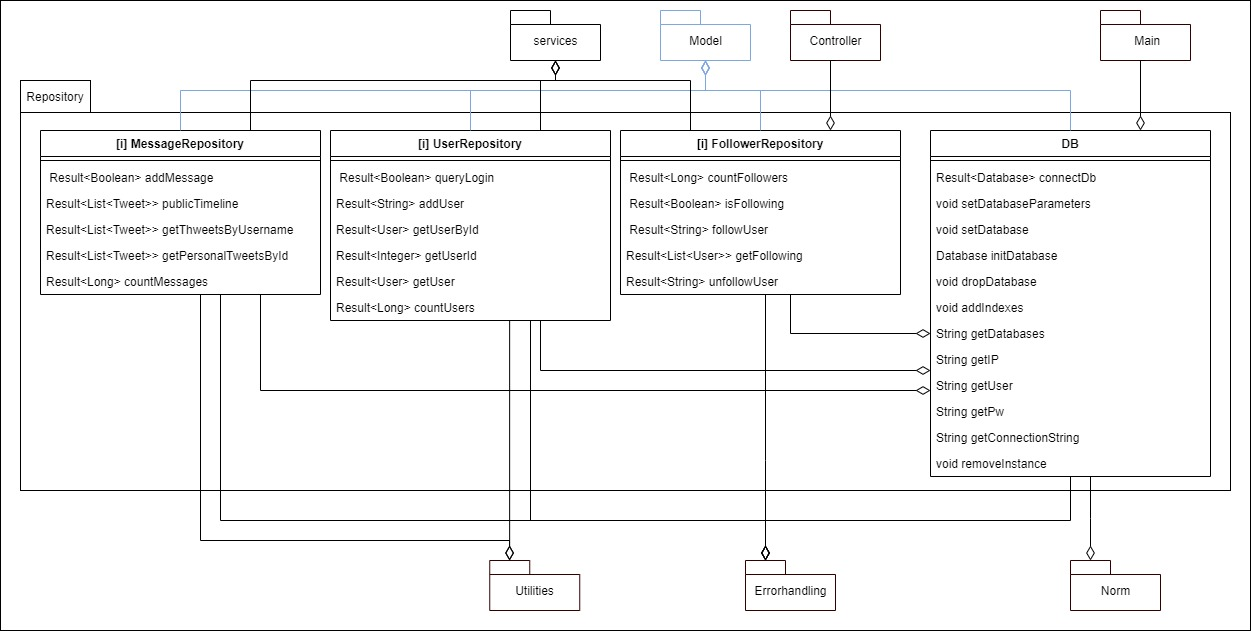
\includegraphics[scale=0.4]{images/class_diagram_repository.jpg}
    \caption{Class diagram repositories, logical view}
    \label{fig:classDiagramRepository}
\end{figure}

\subsubsection{Model}
Model contains classes used by NORM as templates for creating database entities. Class diagram can be seen in \hyperref[fig:classDiagramModel]{figure \ref{fig:classDiagramModel}}.
\begin{figure}[H]
    \centering
    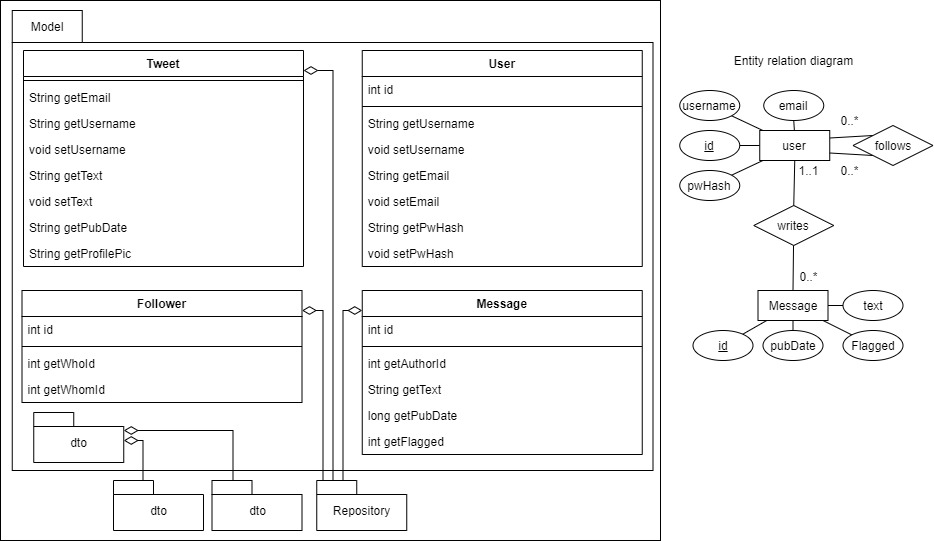
\includegraphics[scale=0.5]{images/class_diagram_model.jpg}
    \caption{On the left is a class diagram for Model, logical view. On the right is an entity relationship diagram.}
    \label{fig:classDiagramModel}
\end{figure}

\subsubsection{Benchmark}
Benchmark is not in deployment and contains code to be run locally only. It is used for measuring the speed of different repository operations and was used to argue for speedups related to extensions to the database, e.g. when indices was added.


\subsection{Dependencies }
\begin{itemize}
    \item \textbf{Spark Java}: A micro framework for creating web applications with minimal effort. %Suitable for the project size and gave us the freedom to structure the application how we wanted it.
    \item \textbf{jinjava}: Template engine based on django template syntax, used to render jinja templates.
    \item \textbf{PicoContainer}: General purpose IoC container.
    \item \textbf{NORM}: Lightweight ORM tool. %that doesn't require the complex markdown files that Hibernate, JPA etc. introduce. Suitable for smaller projects with simple models.
    \item \textbf{MySQL}: Relational database.% Chosen based on familiarity to team members and it's renowned reliability for how long it's been around.  
    \item \textbf{JUnit 5}: Most popular unit-testing framework.
    \item \textbf{Mockito}: Mocking framework with a simple API.
    \item \textbf{SLF4J}: Logging Facade for EFK stack. 
    \item \textbf{prometheus}: Prometheus JVM Client for introducing instrumenting such as gauges, counters and other metrics.
    \item \textbf{org.json}: Toolkit for JSON.
\end{itemize}
\subsubsection{Plugins}
\begin{itemize}
    \item \textbf{Maven}: Build automation tool used to manage Java project and its dependencies.
    \item \textbf{PMD}: Code analyzer, used to find common programming flaws like unused variables, unnecessary object creation etc. 
    \item \textbf{Forbidden API Checker}: Static code analysis that parses java byte code to find invocations of dangerous and deprecated method/class/field signatures. 
    \item \textbf{SonarCloud}: Bug, Vulnerability and Code Smell detection tool with issue contextualization and remediation guidance. Used in our CI for Continuous code inspection.\footnote{\url{https://github.com/DevOps2021-gb/devops2021/wiki/Static-Analysis-Tools}}
\end{itemize}

\subsection{License}
\url{www.licensediscovery.io} was used to analyze Maven dependency licenses. As seen in figure \ref{fig:licenceDep} the strictest license that the majority of dependencies are ruled by is the Apache Software License Version 2. This is the license that we therefore went with.\footnote{\url{https://github.com/DevOps2021-gb/devops2021/blob/main/LICENSE.md}}
\begin{figure}[H]
    \centering
    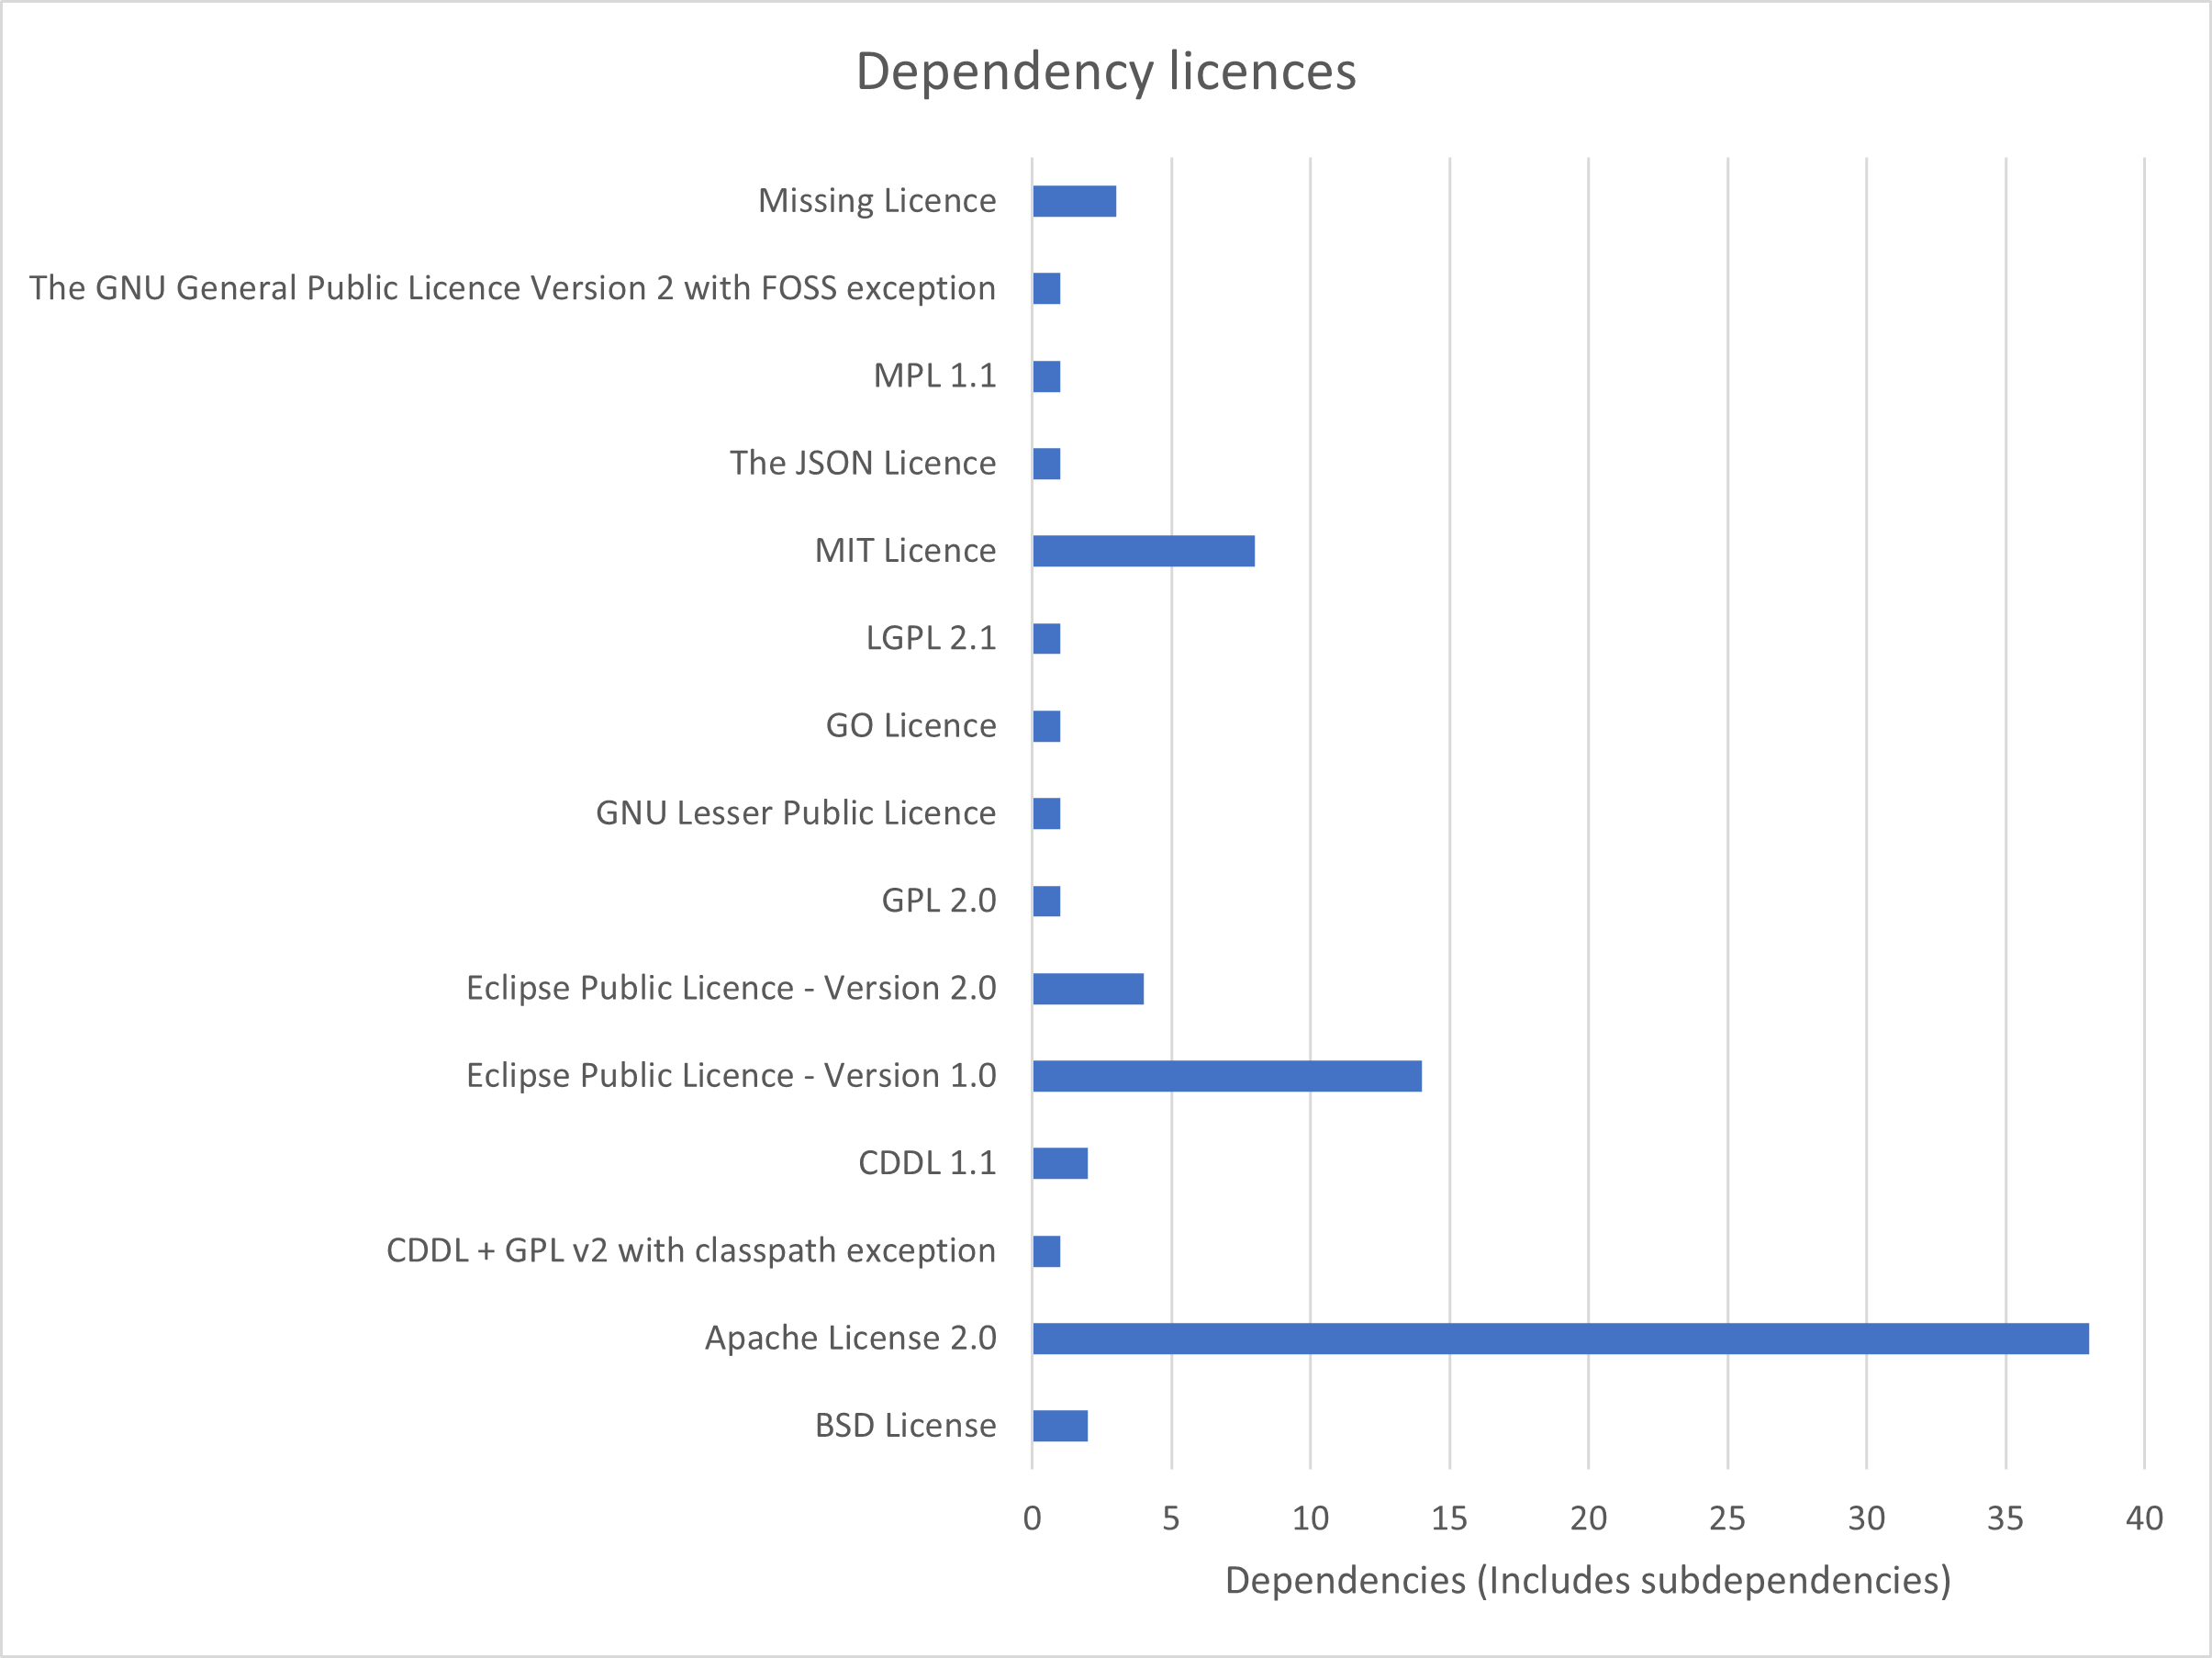
\includegraphics[scale=0.65]{report/images/dependency_licences.png}
    \caption{Overview of dependency licenses. Sub-dependencies included.}
    \label{fig:licenceDep}
\end{figure}
\subsection{Important interactions of subsystem}
\hyperref[fig:componentDiagram]{Figure \ref{fig:communicationDiagram}} shows the interaction between different parts of the system and between users and system.

Code is stored on GitHub, which developers pull and push to during development. When running the code locally, a local database should be used, called \texttt{minitwit}, which runs on port 3306 localhost with password and username "root". The repository contains a docker compose file for running the Minitwit stack locally which includes an empty MySQL database container.

GitHub actions analyze the files pushed using SonarCloud. GitHub Actions deploys to a docker image and pulls down official Prometheus, Grafana, Filebeat, ElasticSearch, Kibana and Nginx images.

The images are all deployed on two DigitalOcean droplets, where the Minitwit containers utilize a remote DigitalOcean database. One droplet is the primary server and uses a floating IP. The other droplet is regarded as a backup and regularly checks through http whether the Minitwit service is responding successfully. If not, the backup droplet obtains the floating IP until the primary is responding as expected. 

The Kibana and Grafana images are for viewing monitoring and logging and the remaining four are for the EFK logging stack.

\begin{figure}[H]
    \centering
    \hspace*{-0.7in}
    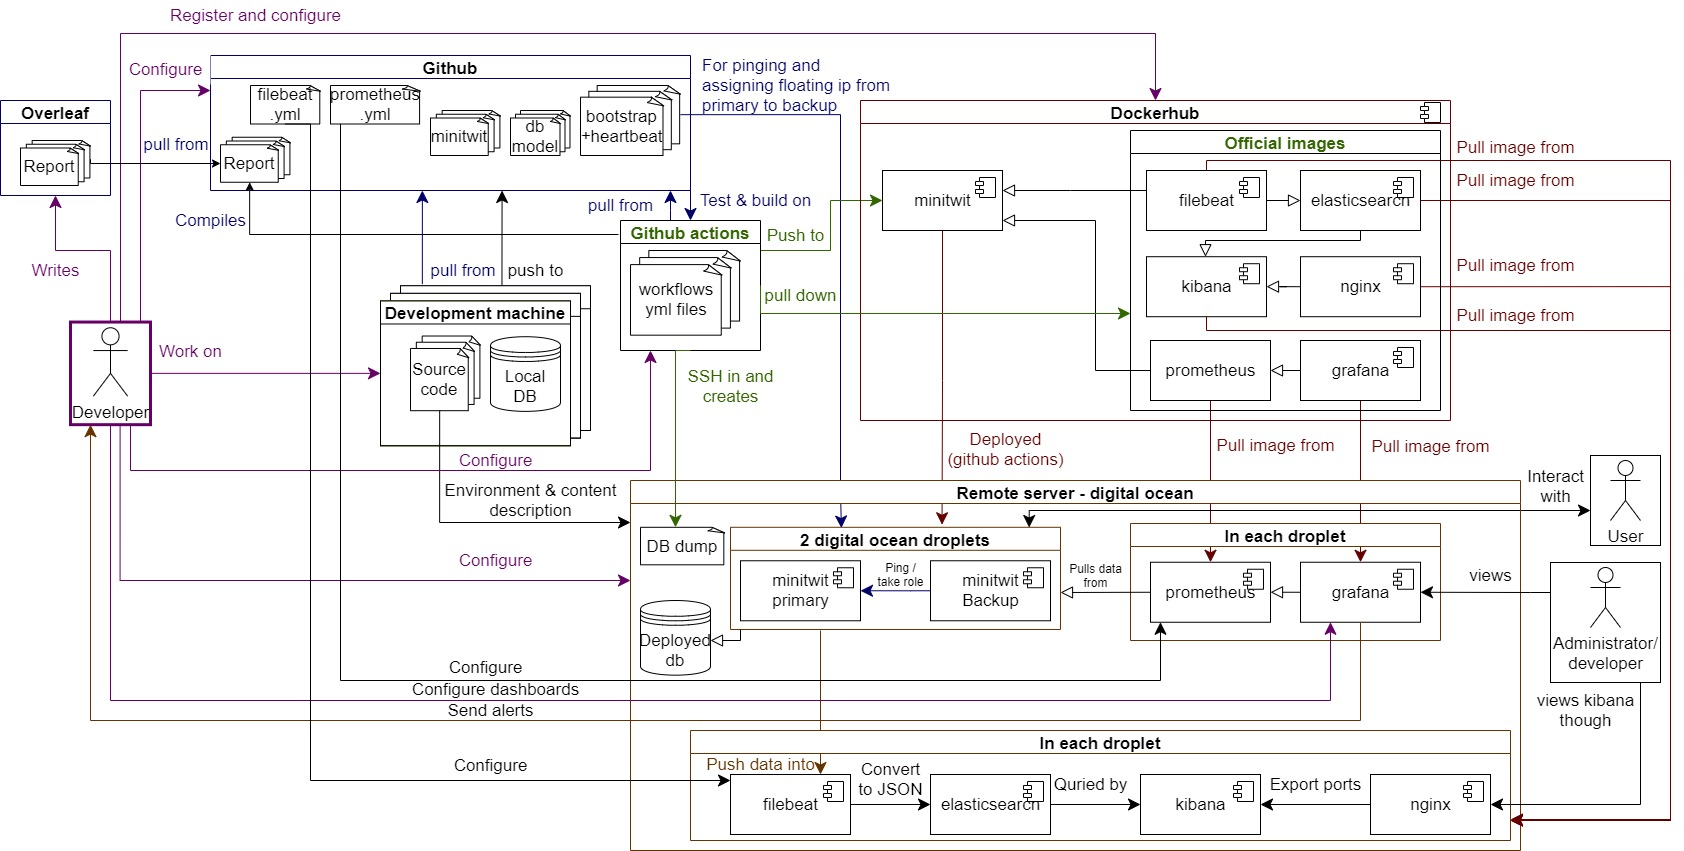
\includegraphics[scale=0.3]{images/Diagrams-Physical_view_deployment_diagram.jpg}
    \caption{Deployment diagram, physical view}
    \label{fig:communicationDiagram}
\end{figure}

\subsection{Current state of system}
The system currently has a single known bug regarding the scaling of the system, see section \ref{issues-operation}. The main tool used for static analysis, Sonarcloud, reports the best rating, \textit{A}, on all measures, with 

\begin{itemize}
    \item 0 bugs
    \item 0 code vulnerabilities and 0 security hotspots
    \item 6 hours technical debt due to 63 code smells
    \item 0.0\% code duplication and 0 duplicated blocks
\end{itemize}

Out of the 63 code smells only 11 are major, critical or blockers and all 63 has been assessed as issues that can be ignored.